% The following choice requires a coordinated choice when PRINTING the report:
%\documentclass[oneside,12pt]{report}  % Use this for one-sided copying (print with printer's normal
%  single-sided option
\documentclass[twoside,12pt,openright]{report}  % You can use this for a slim final printed copy (print with 
%  printer's double-sided option)

% the dimensions of the page
\textheight=9.25in \topmargin=-0.5in   %See note in Chapter 8 of Sample Report about "Page scaling" option in Adobe
\textwidth=6.0in
\oddsidemargin=0.3in
\evensidemargin=0.3in  % Needed to balance even and odd pages in twoside print copy

% Useful packages
\usepackage{amsmath}
\usepackage{tikz}
\usepackage{booktabs}
\usepackage{amsfonts}
\usepackage{amssymb}
\usepackage{amsthm}
\usepackage{float}
\usepackage{textcomp}
\usepackage{algorithmic}
\usepackage{algorithm}
\usepackage{csvsimple} % For csv importing.
\usepackage{arydshln}
\newcommand{\floor}[1]{\left\lfloor #1 \right\rfloor}
%\usepackage[table]{xcolor}
%\usepackage[table,xcdraw]{xcolor}
%\usepackage{tabularx}
\usepackage{lscape}
\usepackage[left=1.1 in, right=1.1 in, top=1 in, bottom = 1 in]{geometry}
\newtheorem{prop}{Proposition}
\newtheorem{theorem}{Theorem}[section]
\newtheorem{lemma}[theorem]{Lemma}
\newtheorem{corollary}[theorem]{Corollary}
\usepackage{graphicx}
\usepackage{lscape}
\newcommand*{\Scale}[2][4]{\scalebox{#1}{\ensuremath{#2}}}%
%\usepackage[dvips]{graphicx} 
\usepackage{doc}
% Following sets up logic and formatting for conditional twoside copying
\usepackage{ifthen, color, fancyvrb}
\usepackage{nextpage}\pagestyle{plain}
\newcommand\myclearpage{\cleartooddpage
  [\thispagestyle{empty}]
  }

%  Set font size for captions
\usepackage[skip=4pt,font=footnotesize]{caption}


\DeclareGraphicsExtensions{ps,eps}
\usepackage{excludeonly}

% If some words are being hyphenated incorrectly, they can be
% given in a list to the \hyphenation command as below.
\hyphenation{ap-pen-dix wer-ther-i-an}

% Theorem-like command definitions:
%\newtheorem{theorem}{Theorem}[chapter]
%\newtheorem{lemma}{Lemma}[chapter]
%\newtheorem{definition}{Definition}  % Note, this italicizes everything

% Print the chapter and sections in the toc
\setcounter{tocdepth}{1}

% Specify which files to typeset for this run (note that overall pagination is preserved)
%\includeonly{chapter1, chapter2}

% Specify which files NOT to typeset for this run (note that overall pagination is preserved)
%\excludeonly{}

% Groundwork for allowing double-sided copying with blank versos
\def\prefacesection#1{
\chapter*{#1}
\addcontentsline{toc}{chapter}{#1}
}


\begin{document}

% Footnote references are symbolized in the front matter, but see below for restoration of numbered footnotes in the body.
\def\thefootnote{\fnsymbol{footnote}}

% The title page is in its own file, ``titlepage.tex''.
% It needs to be edited to reflect information specific
% to your project. 
% don't display the page number
\thispagestyle{empty}

% The numbers below controls the amount of space between the following sections
\def\shiftdowna{0.32in}  % Adjust for balance
\def\shiftdownb{0.22in}  % Adjust for balance

% Set up the boiler plate at the top of the page

\begin{center}
\textbf{{\large Research in Industrial Projects for Students}}\\

\vspace \shiftdowna
%\includegraphics[width=0.4\textwidth]{ipam.eps}\\
% \includegraphics[width=0.4\textwidth]{Graphics/ipamlogo_cmyk_full_lg.eps}\\

\begin{figure}[!ht]
\centering
%\includegraphics[scale=0.2]{images/amd.png}
%\includegraphics[scale=0.02]{images/white.png}
\includegraphics[scale=0.31]{images/ipam.png}
\end{figure}


% SPONSOR
\vspace \shiftdowna
\underline {Sponsor}\\ 
\vspace{5pt}
\textbf{{\large Advanced Micro Devices}} \\
\vspace \shiftdowna
\textbf{Final Report}

% TITLE
\vspace \shiftdowna
\textbf{{\Large Automating Artifact Detection in Video Games}}

% Note the convention used here:  email addresses and urls are typeset in teletype font, colleges are set in italics.

% STUDENTS
\vspace{0.35in}
\underline {Student Members}\\
\vspace{5pt}
 \text{Parmida Davarmanesh} (Project Manager),  \text{\emph{University of Michigan}},\\ 
\vspace{3pt}
\text{\texttt{pdavar@umich.edu}} \\
\vspace{5pt}
\text{Kuanhao Jiang},  \text{\emph{University of Pennsylvania}}  \\
\vspace{3pt}
\text{Tingting Ou},  \text{\emph{Johns Hopkins University}}  \\
\vspace{3pt}
\text{Artem Vysogorets}, \text{\emph{University of Massachusetts Amherst}}  \\

% ACADEMIC MENTORS
\vspace \shiftdownb
\underline {Academic Mentor} \\
\vspace{5pt}
\text{Shantanu Joshi}, \text{\texttt{s.joshi@g.ucla.edu}} 

% SPONSORS
\vspace \shiftdownb
\underline {Sponsoring Mentors}\\
\vspace{5pt}
\text{Nicholas Malaya}, \text{\texttt{nicholas.malaya@amd.com}} \\
\vspace{3pt}
\text{Max Kiehn}, \text{\texttt{max.kiehn@amd.com}}  \\
\vspace{3pt}
\text{Alan Lee}, \text{\texttt{alan.lee@amd.com}} 

% CONSTULANTS (comment out this text if there are no consultants)
% \vspace \shiftdownb
% \underline {Consultants}\\
% \vspace{5pt}
% $\langle \text{Name}\rangle$\\
% \vspace{3pt}
% $\langle \text{Name}\rangle$

% DATE
\vspace \shiftdowna
\text{Date: August 19, 2019}\\

\vspace \shiftdowna



\end{center}

\vfill  %Fill page to force following note to bottom
\footnoterule
\noindent \small{This project was jointly supported by \text{AMD}  and NSF Grant $\langle \text{DMS} \rangle$ 1440415.}



% Begin ABSTRACT
\ifthenelse{\boolean{@twoside}}{\myclearpage}{}
\prefacesection{Abstract}

% don't display the page number
%\thispagestyle{empty}



\vspace{24pt}


The video game industry is the most influential form of entertainment in America, producing \$43B in revenue in 2018. Regardless of how advanced the gaming hardware and software are, gameplay is often tainted with graphics errors and screen artifacts. Currently, artifact detection is a labor intensive process, where artifacts are reported individually by users who experience them. Further, there is currently a lack of consolidated framework for systematically cataloging and analyzing graphics corruptions. \\

\noindent
This project intends to apply machine learning to the creation of an automated software that is capable of detecting graphics corruptions in video games. Given a limited sample of corruption examples provided by our sponsoring company, Advanced Micro Devics (AMD), 13 most common screen artifacts were identified, described and recreated using Python programming language. We then created a dataset of 50,000 frames consisting of both normal gameplay frames as well as synthetically obtained corrupted frames of 12 different types. Feature representation of the data included discrete Fourier transformation, histogram of oriented gradients and graph Laplacian. Various combinations of these features were used to train machine learning models that identify individual classes of graphics corruptions and that later were assembled into a single mixed experts ``ensemble'' classifier. The ensemble classifier was tested on heldout test sets, and produced an accuracy of 84\% on the games it had seen before, and 69\% on games it had never seen before.


%The video game industry is the most influential form of entertainment in America. Regardless of how advanced the gaming hardware and software are, gameplay is often tainted with graphics errors and screen artifacts which are labor intensive to detect and fix. In this research, we have automated the process of anomaly detection and classification by developing machine learning models that are able to label each frame of a video game as glitched or normal. Since this has never been done before, there is a lack of labeled and catalogued gaming data. we first generated our own database by extracting gaming images from gameplay videos and added realistic-looking artifacts to those images. Then we explored various ways to extract features from the images, such as Fourier transform, the histogram of gradients and the graph Laplacian. Using the extracted features, we built eleven classifiers to detect different types of glitches respectively. Combining the individual classifiers through a logistic regression, we constructed an ensemble model to detect all eleven types of glitches.



% Begin ACKNOWLEDGMENTS
\ifthenelse{\boolean{@twoside}}{\myclearpage}{}
\prefacesection{Acknowledgments}


\begin{quote}
We wish to express our gratitude to the Institute of Pure and Applied Mathematics and, in particular, to Dima Shlyakhtenko, Susana Serna and Dimi Mavalski for hosting, funding and organizing the RIPS 2019 program.
\\\hspace{\fill}\\
We also thank our industry mentors, Nicholas Malaya, Max Kiehn and Alan Lee for shedding light on and helping us get through the challenges posed by the project.
\\\hspace{\fill}\\
Our team is especially thankful to our academic mentor, Shantanu Joshi, who has been continuously providing us with guidance, support and critical ideas. Without his vision and dedication this research would not have been possible.
\end{quote}



%%



% Table of contents, List of Figures, and List of Tables.
\ifthenelse{\boolean{@twoside}}{\myclearpage}{}
\tableofcontents

\ifthenelse{\boolean{@twoside}}{\myclearpage}{}
\listoffigures

\ifthenelse{\boolean{@twoside}}{\myclearpage}{}
\listoftables

% matter, and use arabic numerals for footnotes in the body
\renewcommand{\thefootnote}{\arabic{footnote}}
\setcounter{footnote}{0}

% Chapter 1 -- the Introduction
\ifthenelse{\boolean{@twoside}}{\myclearpage}{}
\chapter{Introduction}\label{Ch:Introduction}

Founded in 1969 as a Silicon valley start-up, Advanced Micro Devices (AMD) is an American company specializing in semiconductor products such as microprocessors, motherboard chipsets and graphic processors. With these products, AMD brings advances in high-performance computing to both IT businesses and consumer markets. In particular, Graphic Processing Units (GPUs) developed and manufactured by AMD empower numerous modifications of gaming consoles including Xbox and PlayStation, thereby contributing to the fast growing gaming industry.\\
\\
According to the statistics published by the Entertainment Software Association, more than 65\% of Americans play video games on at least one type of device \cite{stats}. Furthermore, in 2018 alone, the video game industry produced a revenue of \$43B, an 18\% growth from 2017 \cite{growth}. Therefore, in light of the increasing market share of AMD GPUs---the power source for most gaming devices---it is in AMD's interest to ensure high-quality and error-free gameplay. While games may contain issues of many different sorts, graphics corruption and visual artifacts constitute among the major complaints of users. These artifacts occur as software or hardware errors that alter visual appearance of the game or its individual frames. Figure \ref{fig:bugs} shows some examples of such corruptions as provided by AMD.

\begin{figure}[h]
\centering
\includegraphics[scale=0.56]{images/bug1new.png}
\includegraphics[scale=0.283]{images/bug2new.jpg}\\
\includegraphics[scale=0.28]{images/bug3new.jpg}
\includegraphics[scale=0.28]{images/bug4new.jpg}\\
\vspace{5pt}
\caption[Examples of video game artifacts]{Examples of video game artifacts (images are courtesy of AMD).}
\label{fig:bugs}
\end{figure}

\noindent
Currently, the task of artifact detection or correction is manual; users report corrupted images to developers or post them in blogs and online forums. Hence, publicly available data is extremely limited, while machine learning algorithms require large datasets for successful training. \\

\noindent In Chapter \ref{Ch:datagen}, we describe our approach at obtaining ``synthetic'' corrupted images using a newly created ``Glitchify'' software that adds certain types of graphics artifacts to normal images. This program was carefully designed to produce 13 different kinds of artifacts that are assumed to occur most frequently. Extraction of relevant features (preprocessing) from the produced data is performed in Chapter \ref{Ch:feature}. Given the characteristics of the 13 artifacts considered in this study, we focused on the discrete Fourier transform, graph Laplacian and pixel-wise anomaly measures. Chapter \ref{Ch:classification} describes designs of models that identify each of the 13 different types of corruptions as well as the assembly of the final ``ensemble'' classifier. Finally, in Chapter \ref{Ch:results} we cover the results that we obtained from our classifiers, yielding a 69\% accuracy on a heldout test set where the games have never been seen by any of the models. We will then wrap up with a discussion of the results and possible sources of bias in Chapter \ref{Ch:discussion}.


\endinput


% Chapter 2
\ifthenelse{\boolean{@twoside}}{\myclearpage}{}
\chapter{Data Generation}\label{Ch:datagen}

Automating artifact detection requires large amounts of data (i.e. corrupted frames), which is extremely limited. Therefore, it was critical that we generate our own data that will well represent the actual distribution of corrupted images. The prototype for our ``synthetic'' data was a sample of about 20 images provided by AMD that were claimed to be representative of artifacts seen most frequently (see Figure \ref{fig:bugs}). The \texttt{Glitchify} software was then produced to artificially create images with different types of corruptions seen in the sample set. Unlike artifacts shown in Figure \ref{fig:bugs}, some of the images in the sample appeared to have highly content-related artifacts, which would be infeasible to reproduce without using laborious segmentation methods. For example, the leftmost image in Figure \ref{fig:hard} exhibits a warrior with a missing corpus, however, some elements of his armor are displayed. The other picture in Figure \ref{fig:hard} contains a car with missing color textures. Since recreating such artifacts would have required object recognition techniques, this study did not address such content-related corruptions.

\begin{figure}[H]
\centering
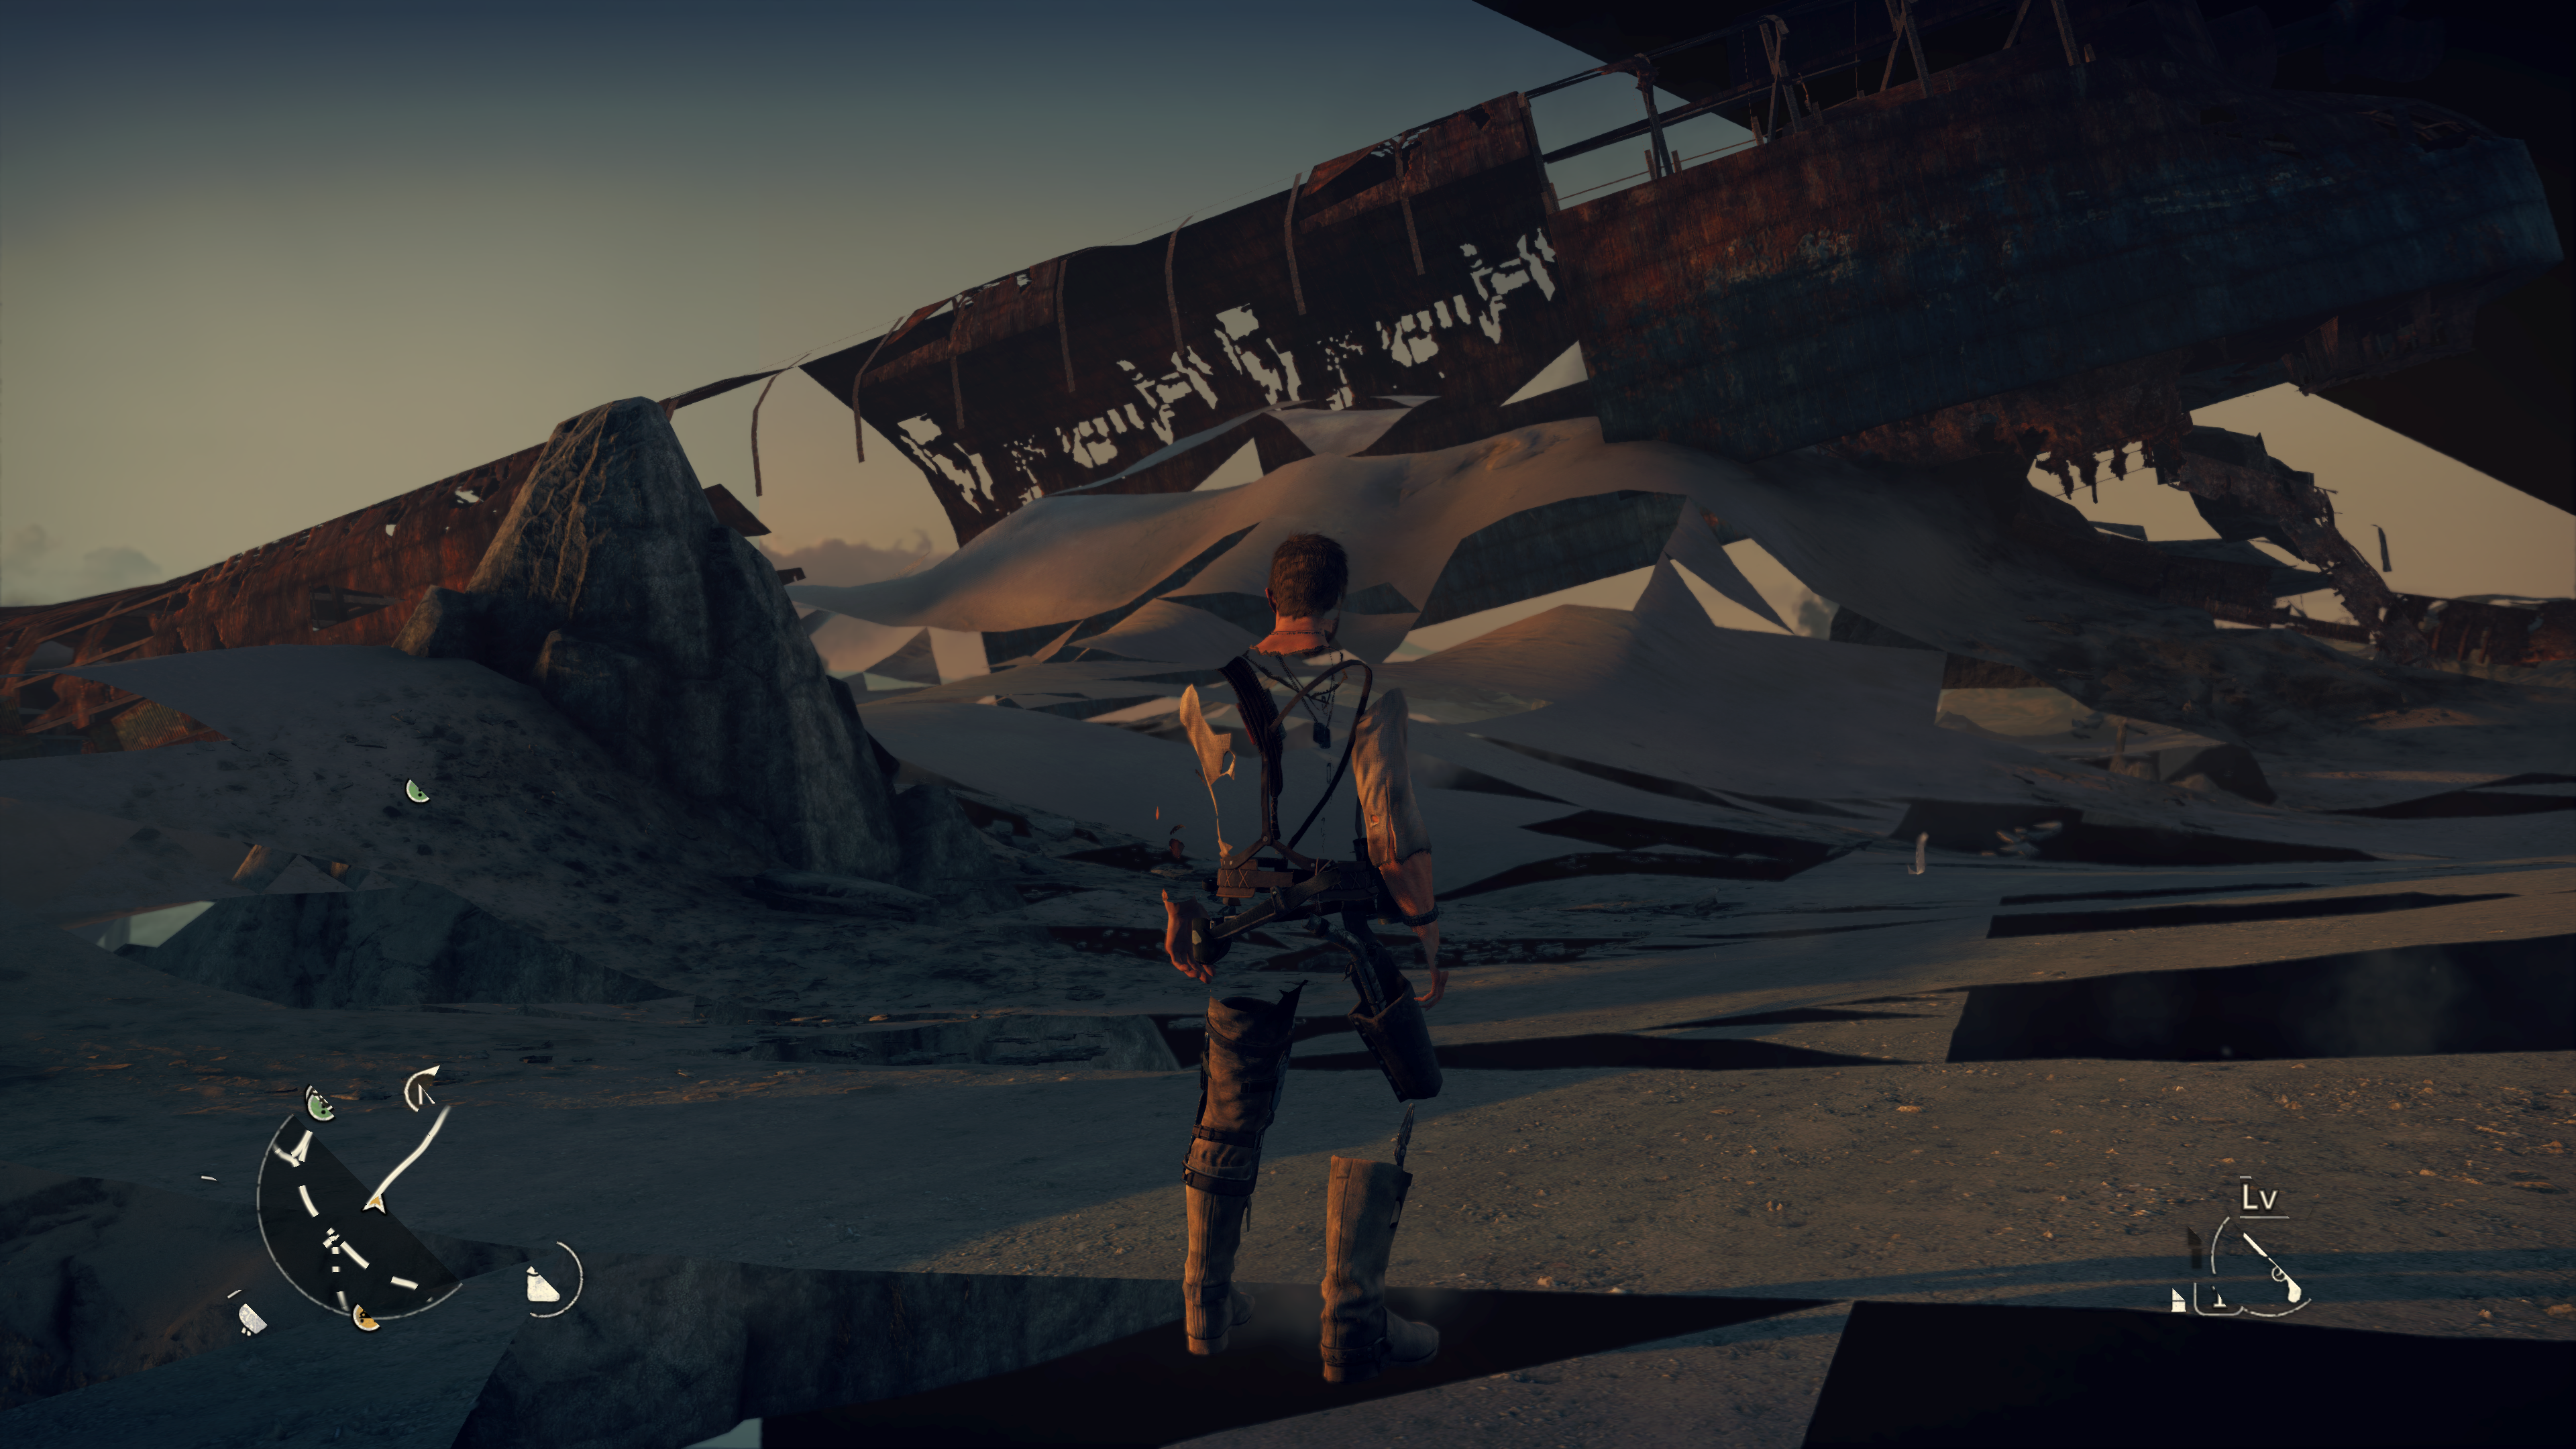
\includegraphics[scale=0.086]{images/hard1.png}
\includegraphics[scale=0.181]{images/hard2.png}
\vspace{5pt}
\caption[Examples of content-related artifacts]{Examples of content-related artifacts (images are courtesy of AMD).}
\label{fig:hard}
\end{figure}
\noindent
In order to manually reproduce different artifacts, we defined 13 classes of corruptions based on their appearance.
In the following sections, we will describe each artifact in detail.

\section*{Shader}
Shader is a program within GPU that governs frame rendering and determining various surface properties such as texture, reflection and lightning \cite{shader}. We define a class of corruptions---\textit{shader} artifacts, which are assumed to be caused by an incorrect operation of this program. Typically, shader artifacts are marked by the presence of polygonal shapes of a few different colors blended together or fading into transparency (see Figure \ref{shader}). This type of corruption was reproduced in Figure \ref{shader}.
\begin{figure}[H]
\centering
\includegraphics[scale=0.135]{images/shader1.png}
\includegraphics[scale=.42]{images/shader2.jpg}
\vspace{5pt}
\caption[shader artifacts]{shader corruption: actual (left) and reproduced with \texttt{Glitchify} (right).}
\label{shader}
\end{figure}
\section*{Shapes}
Unwanted random polygonal \textit{shapes} are also common in video games, especially in first-person shooting games. By inspection of the sample images, we conclude that shapes tend to appear in the darker part of the frame. The corrupted image provided by AMD shown in Figure \ref{fig:shapes} on the left exhibits thin black triangles that emanating from the center. To reproduce this artifact, \texttt{Glitchify} adds mono-colored polygonal shapes to the darkest region of the input image as shown on the right in Figure \ref{fig:shapes}.
\begin{figure}[H]
\centering
\includegraphics[scale=0.405]{images/shapes1.jpg}
\includegraphics[scale=0.43]{images/shapes2.jpg}
\vspace{5pt}
\caption[Shape artifacts]{shapes corruption: actual (left) and reproduced with \texttt{Glitchify} (right).}
\label{fig:shapes}
\end{figure}
\section*{Discoloration}
Another type of graphic artifact is \textit{discoloration}. As shown in the real corrupted image of Figure 2.4, the light spots of the image, which is a screenshot of game \textit{Civilization VI} become blue. The reason behind this phenomenon might be data overflow -- if we have an integer color value greater than 255, say 256, it will be cast back to 0. To produce a similar visual artifact, we randomly change the color of any pixel whose intensity exceeds a certain threshold. In our reproduced example image of Figure 2.4, the bright spots are painted white. We can choose the threshold to be based on the red, green or blue channel, or the overall intensity.

\begin{figure}[!ht]
\includegraphics[scale=0.132]{images/disco1.jpg}
\includegraphics[scale=0.152]{images/disco2.png}
\vspace{5pt}
\caption[Discoloration artifacts]{Discoloration artifacts: real corrupted image provided by AMD (left) and our reproduced corrupted image (right).}
\label{fig:discoloration}
\end{figure}

\section*{Random Patches}
The picture below on the left side illustrates the artifact of \textit{random patches}. In this particular image, the glitches are the small blue patches on the wall and the floor. The patches are usually part of an object, for example the wall. To reproduce this visual artifact, our program adds a random number of patches of random color and position to the image. We use segmentation algorithms \cite{watershed} to detect contours of objects so that the patches cover only part of a single object and do not lie on the edges of objects.

\begin{figure}[!ht]
\includegraphics[scale=0.128]{images/rp1.jpg}
\includegraphics[scale=0.16]{images/rp2.png}
\vspace{5pt}
\caption[Random patches artifacts]{Random patches artifacts: real corrupted image provided by AMD (left) and our reproduced corrupted image (right).}
\label{fig:rp}
\end{figure}

\section*{Dotted Lines}
In some corrupted images, we may also observe \textit{dotted lines}. For instance, in Figure 2.6 below, we can observe black dotted lines in the leftmost picture. This visual artifact is often hard to recognize unless we zoom-in on the corrupted picture. Our program includes two different methods to produce dotted-line artifacts. We either just add several dotted lines of random color and slope to the input frames, or we can have radial lines emanating from a single point.

%%%%%%%%
\newpage
%%%%%%%

\begin{figure}[!ht]
\includegraphics[scale=.35]{images/dl1.png}
\includegraphics[scale=.25]{images/dl2.png}
\includegraphics[scale=.45]{images/dl3.png}
\vspace{5pt}
\caption[Dotted line artifacts]{Dotted line artifacts: real corrupted image provided by AMD (leftmost), our reproduced corrupted image with random lines of green color (middle) and radial lines of red color (rightmost).}
\label{fig:dl}
\end{figure}


\section*{Parallel Lines}
In the screenshot of the League of Legends game (Figure \ref{fig:pl}), there are \textit{parallel lines} glitches. The color of the line segment is the pixel color of the starting point of the line. The method to generate parallel lines, clearly, is to add a random number of parallel lines whose colors are determined by the starting points.

\begin{figure}[!ht]
\includegraphics[scale=.2025]{images/pl1.jpg}
\includegraphics[scale=.135]{images/pl2.png}
\vspace{5pt}
\caption[Parallel line artifacts]{Parallel line artifacts: real corrupted image provided by AMD (left) and our reproduced corrupted image (right).}
\label{fig:pl}
\end{figure}


\section*{Square Patches}
Occasionally, gamers observe small \textit{square patches}, often with bright, blotches of color during gameplay. The square patches of the real glitched image provided by AMD (Figure 2.8) are purple or blue as highlighted in the red rectangle. To reproduce this glitch, we place some little square patches of random color on the input pictures. Our reproduced corrupted image on the right has cyan-blue square patches, highlighted in the red rectangle as well.
%%%%%%%%%%%%%%
\newpage
%%%%%%%%%%%%%

\begin{figure}[!ht]
\includegraphics[scale=0.64]{images/sp1.png}
\includegraphics[scale=0.32]{images/sp2.png}
\vspace{5pt}
\caption[Square patches artifacts]{Square patches artifacts: real corrupted image provided by AMD (left) and our reproduced corrupted image (right).}
\label{fig:sp}
\end{figure}



\section*{Texture Pop-in}
In computer graphics, textures are used extensively and are very important for rendering realistic 3-D images. \textit{Texture pop-in} refers to textures not loading in time or not loaded correctly. As a result, low-resolution textures appear instead of the high-resolution ones that gamers are expecting to see. To reproduce the texture pop-in artifact, we randomly select a region of the input image and then blur it by applying a Gaussian filter.

\begin{figure}[!ht]
\includegraphics[scale=0.32]{images/tp1.png}
\includegraphics[scale=0.425]{images/tp2.png}
\vspace{5pt}
\caption[Texture pop-in artifacts]{Texture pop-in artifacts: real corrupted image provided by AMD (left) and our reproduced corrupted image (right). The blurry regions due to texture-pop in are highlighted using red rectangles in both images.}
\label{fig:tp}
\end{figure}



\section*{Triangulation}
Some gamers have reported \textit{triangulation} artifacts \footnote{https://forums.warframe.com/topic/1095994-sanctuary-conduit-pixelated-screen-bug/}. These typically occur in intensive 3D games, where surfaces are rendered by numerous little triangles that form triangle meshes. Due to graphics defects, such triangular meshes are either displayed at a coarse resolution or displayed by sharp incorrectly colored triangles instead of smooth representations of surfaces. We developed two methods to reproduce this visual artifact. The first is regular triangulation, illustrated by the picture in the bottom left corner of Figure 2.10. To accomplish this, we randomly select a region which is then  divided into right triangles. The color of each triangle is determined by the weighted average of pixel colors within the triangle. The second is random triangulation, where we divide the regions into random triangles instead of right triangles using Delaunay triangulation\cite{delauny}.


\begin{figure}[!ht]
\includegraphics[scale=.152]{images/tri1.png}
\includegraphics[scale=.152]{images/tri2.png}\\
\includegraphics[scale=.13]{images/tri3.png}
\includegraphics[scale=.13]{images/tri4.png}
\vspace{5pt}
\caption[Triangulation artifacts]{Triangulation artifacts: real corrupted image found online (top row), our reproduced corrupted image with regular triangulation (bottom left) and random triangulation (bottom right).}
\label{fig:tri}
\end{figure}


\section*{Line Pixelation}
\textit{Line pixelation} is a peculiar type of gaming artifact that can have both subtle or pronounced effects. Through careful inspection of the left image in Figure \ref{fig:lp}, one can spot the line pixelation artifact at the very bottom of the picture. In order to capture the distribution (pixel intensity variations) in this kind of artifact, we inserted a random number of noisy stripes with random orientations and positions.

\begin{figure}[!ht]
\includegraphics[scale=0.143]{images/lp2.png}
\includegraphics[scale=.836]{images/lp1.png}
\vspace{5pt}
\caption[Line pixelation artifacts]{Line pixelation artifacts: real corrupted image provided by AMD (left) and our reproduced corrupted image (right).}
\label{fig:lp}
\end{figure}


\section*{Screen Stuttering}
Screen \textit{stuttering} was one of the most interest artifacts to figure out. The image on the top left of Figure \ref{fig:stuttering} is the corrupted image we received from AMD. We first had to figure out what the normal image looked like before we could reproduce this artifact. The image on the top right shows what one of our team members cleverly did to figure out the normal image. We discovered that screen stuttering occurs when neighboring columns and rows of the image are swapped. In this way we were able to recover the original image (bottom left), and then reproduce this artifact (bottom right).

\begin{figure}[!ht]
\centering
\includegraphics[scale=0.29]{images/stutter1.png}
\includegraphics[scale=0.458]{images/stutter2.png}
\includegraphics[scale=0.68]{images/stutter.png}
\includegraphics[scale=0.11]{images/stutter3.jpg}
\vspace{5pt}
\caption[Screen stuttering artifacts]{Screen stuttering artifacts: real corrupted image provided by AMD (top left) and our reproduced corrupted image (bottom right).}
\label{fig:stuttering}
\end{figure}

\section*{Screen Tearing}
One of the most common gaming artifacts is \textit{screen tearing}. Screen tearing occurs when two consecutive frames in a video get rendered into the same image. Therefore, part of the image shows the scene at a certain point in time, while the other part of the same image shows that scene at a later time. In order to reproduce this type of artifact, we select two frames in a video that are 100 frames apart from each other, and then randomly replace some rows (or columns) of the first frame with the corresponding rows (or columns) of the second frame. Examples are shown in Figure \ref{fig:tearing}.

%%%%%%%%%%%%%%%%%%
%%%%%%%%%%%%%%%%%%
\newpage
%%%%%%%%%%%%%%%%%%
%%%%%%%%%%%%%%%%%%

\begin{figure}[!h]
\includegraphics[scale=0.29735]{images/tearing1.jpg}
\includegraphics[scale=0.627]{images/tearing2.png}
\vspace{5pt}
\caption[Screen tearing artifacts]{Screen tearing artifacts: real corrupted image provided by AMD (left) and our reproduced corrupted image (right).}
\label{fig:tearing}
\end{figure}


\section*{Morse Code Pattern}

\textit{Morse code} pattern (shown in Figure \ref{fig:morse}) appears when memory cells on a graphic card become stuck and display their stuck values on the screen rather than displaying the true image. Over-clocking and over-heating are two possible causes of such memory corruption. Over-clocking refers to the action of running a GPU at a higher speed than it is designed to run, and over-heating refers to running a GPU such that its temperature exceeds its maximum specified operating temperature. In order to reproduce this type of artifact, we add morse-code-like patterns to random locations in the frame, as shown in Figure \ref{fig:morse}.

\begin{figure}[!h]
\includegraphics[scale=0.765]{images/morse1.png}
\includegraphics[scale=0.288]{images/morse2.png}
\vspace{5pt}
\caption[Morse code artifacts]{Morse code artifacts: real corrupted image extracted from online YouTube video (left) and our reproduced corrupted image (right).}
\label{fig:morse}
\end{figure}


\section*{Glitchify Software}
% \textcolor{red}{Add the software interface here}. \textcolor{red}{You don't have to discuss all the options, but give a few examples. Also use the textt font to show code.}

\noindent In order to generate a large number of corrupted images, we implemented a software named ``Glitchify" that takes in images and videos and outputs corrupted images. The software interface is shown in Table \ref{interface}.
\begin{center}
\begin{table}
\scalebox{0.87}{
\begin{tabular}{ |c|c| } 
 \hline
 Input Argument & Description \\ 
  \hline
 "Input" & Path to the directory that contains input images and/or videos. \\ 
  \hline
 "Output" & Path to the directory where output images are saved. \\ 
 \hline
  "Artifact Type" & Type of artifact to be inserted to the input images/videos.\\ 
   \hline
   "Interval" & Number of frames skipped before the next frame where artifacts are inserted.\\
   \hline
   "Output Array" & Whether to output the corrupted images in the format of numpy array.\\
      \hline
      "Resize Output" & Whether to resize the corrupted images to a specified size.\\
    \hline
\end{tabular}}
\caption{\label{interface}Interface of the \textit{Glitchify} software.}
\end{table}
\end{center}
\subsection*{Generating Training, Testing, and Holdout datasets}

\noindent We used the newly created \texttt{Glitchify} program to generate these artifacts and obtained a large dataset. \\


\noindent In order to achieve this, we downloaded long (2-6 hour) gameplays of different video games. We then extracted around 2,000 images from each game until we had a total of 50,000 images. We manually scanned the extracted frames to ensure that they are not already corrupted to the best of our abilities. This was a cumbersome and error prone process as we had to make (subjective) decisions as to whether the features we were seeing in some frames were part of the gameplay experience or not. For example, the two images illustrated in Figure \ref{fig:hard} are examples of frames where it is not clear whether they are corrupted or normal. We made an effort to exclude all the images that were ambiguous from our data set. After extracting normal images, we then created a uniform distribution of different kinds of artifacts with half of the images, leaving the other half intact as ``normal" images. \\

\begin{figure}
\centering
\includegraphics[scale=0.11]{images/line_pixelation_39.png}
\includegraphics[scale=0.11]{images/line_pixelation_68.png}
\caption{Examples of frames that are hard to label}
\label{hard}
\end{figure}


\noindent Since we extracted high-quality images (1920 pixels x 1080 pixels x 3 color channels), the dimensions of the images were too large to be used by our models. We often experienced unexpected memory error when we loaded the images in our programs, and we did not have enough RAM to feed the original sized images into our models. Additionally, nearby pixels in images are often related, therefore by feeding an entire image into a model we are giving it a lot of repetitive information. Our solution to this problem was to use various feature representations of the images, whose dimensions are much smaller than those of the original images. In the next chapter we will discuss the features that we considered.

\begin{table}[h]
\centering
\includegraphics[scale=0.8]{tables/games.pdf}
\caption{Games from which the images were extracted.}
\label{games}
\end{table}


\endinput


% Chapter 3
\ifthenelse{\boolean{@twoside}}{\myclearpage}{}
\chapter{Feature Extraction}\label{Ch:feature}
% \begin{document}


%\section{Feature Extraction}

\section{Fourier Transformation}
The Fourier transformation converts signals from spatial domain to frequency domain and vice verse. The two-dimensional Discrete Fourier Transform (DFT) is used to process two-dimensional discrete signals such as images \cite{Cooley}. Given a one-channel signal $f(x,y)$ with dimensions $M\times N$, its DFT $F(u,v)$ is given by
\begin{align}
F(u,v)=\frac{1}{\sqrt{MN}}\sum\limits_{x=0}^{M-1}\sum\limits_{y=0}^{N-1}f(x,y)e^{-2i\pi\frac{ux}{M}}e^{-2i\pi \frac{vy}{N}},
\end{align}
where $0\leqslant u\leqslant M-1$ and $0\leqslant v\leqslant N-1$ are the spectral coordinates \cite{Burger}. However, for visualization purposes, we shift the zero frequency $(0,0)$ to the center $(\frac{m}{2},\frac{n}{2})$ of the image so that $-\lfloor\frac{M}{2}\rfloor\leqslant u\leqslant \lfloor\frac{M-1}{2}\rfloor$ and $-\lfloor\frac{N}{2}\rfloor\leqslant v\leqslant \lfloor\frac{N-1}{2}\rfloor$. The original signal can be extracted from $F(u,v)$ with
\begin{align}
f(x,y)=\frac{1}{\sqrt{MN}}\sum\limits_{u=0}^{M-1}\sum\limits_{v=0}^{N-1}F(u,v)e^{2i\pi\frac{ux}{M}}e^{2i\pi \frac{vy}{N}}.
\end{align}
The rationale behind considering DFT as a feature for the graphics artifact classification is that several types of graphics (e.g. morse code, parallel lines, etc.) exhibit periodic patterns that could be best identified in the frequency domain. Previous studies provide evidence of successful application of this technique to the detection of periodic patterns in signals \cite{russians}. Additionally, most graphics corruptions have sharp edges and fine structure, which finds reflection in the high-frequency components. For example, Figures \ref{fig:fourier1}, \ref{fig:fourier2}, \ref{fig:fourier4} and \ref{fig:fourier3} show the Fourier transformation of the ``Borderlands 2'' game screenshot with different graphics artifacts added. Note that intensities represent log-transformed absolute values of the corresponding DFT descriptors.
\begin{figure}[H]
\centering
\includegraphics[scale=0.11]{images/bd.jpg}
\includegraphics[scale=0.11]{images/bd-14-ft.png}\\\hspace{\fill}\\[-2ex]
\caption[Fourier transform]{Normal image (left) and its DFT (right).}
\label{fig:fourier1}
\end{figure}
\begin{figure}[H]
\centering
\includegraphics[scale=0.11]{images/experiment10.png}
\includegraphics[scale=0.11]{images/experiment11.png}\\\hspace{\fill}\\[-2ex]
\caption[Fourier transform on morse code artifact]{Image with the morse code artifact added (left) and its DFT (right).}
\label{fig:fourier2}
\end{figure}
\begin{figure}[H]
\centering
\includegraphics[scale=0.11]{images/0_stuttering.png}
\includegraphics[scale=0.11]{images/stuttering.png}\\\hspace{\fill}\\[-2ex]
\caption[Fourier transform on stuttering artifact]{Image with the stuttering artifact added (left) and its DFT (right).}
\label{fig:fourier4}
\end{figure}
\begin{figure}[H]
\centering
\includegraphics[scale=0.11]{images/0_shape.png}
\includegraphics[scale=0.11]{images/shape.png}\\\hspace{\fill}\\[-2ex]
\caption[Fourier transform on stuttering artifact]{Image with the stuttering artifact added (left) and its DFT (right).}
\label{fig:fourier3}
\end{figure}\hspace{\fill}\\
Figure \ref{fig:fourier1} displays an image without defects and its DFT. As seen from Figure \ref{fig:fourier2}, even minor corruptions that are rather imperceptible visually have a substantial effect on the image's DFT. Figures \ref{fig:fourier4} and \ref{fig:fourier3} illustrate the explicit patterns in the image's DFT after other types of artifacts are added to the original frame.\\\hspace{\fill}\\
Most screen artifacts affect the high frequency components of the DFT. Hence, we considered adopting another feature that is constructed from high frequencies of the image spectrum. In particular, we transform the DFT $F(u,v)$ with a high-pass filter to obtain 
\begin{align}
\widetilde{F}(u,v)=\begin{cases} 
      F(u,v) & \lfloor\frac{M}{2}\rfloor-100\leqslant u\leqslant \lfloor\frac{M}{2}\rfloor+100, \lfloor\frac{N}{2}\rfloor-100\leqslant v\leqslant \lfloor\frac{N}{2}\rfloor+100 \\
      0 & \text{otherwise},
   \end{cases}
\end{align}
where original coordinates $0\leqslant u\leqslant M-1$ and $0\leqslant v\leqslant N-1$ are used. The resulting signal $\widetilde{F}(u,v)$ is then brought back to spatial domain to become our new feature $\widetilde{f}(x,y)$  (see Figures \ref{fig:fourier5}, \ref{fig:fourier6}).
\begin{figure}[H]
\includegraphics[scale=0.11]{images/pixelationv1.png}
\includegraphics[scale=0.11]{images/pixv1-ft.png}\\
\caption[Fourier transform on stuttering artifact]{Corrupted image $f(x,y)$ (left) and its DFT $F(u,v)$ (right).}
\label{fig:fourier5}
\end{figure}
\begin{figure}[H]
\includegraphics[scale=0.11]{images/pixv1-corn.png}
\includegraphics[scale=0.11]{images/pixv1.png}\\
\caption[Fourier transform on stuttering artifact]{High-pass filtered DFT $\widetilde{F}(u,v)$ and its inverse $\widetilde{f}(x,y)$ (right).}
\label{fig:fourier6}
\end{figure}

% Talk about high frequencies and the other feature.

\section{Histogram of Oriented Gradients (HoG)}

Histogram of oriented gradients is a feature used in computer vision to detect objects in an image \cite{1467360}. The steps to compute the HoG feature are shown as follows:\\


\noindent An $M \times N$ color image can be represented using three functions $R,G,B : \mathbb{R}^{M \times N} \rightarrow R$ that map each coordinate to the corresponding red, green, and blue color intensity value, respectively. The gradient of the functions at each coordinate can be approximated by applying discrete derivative masks $[-1,0,1]$ and $[-1,0,1]^T$ at each coordinate. Sometimes different derivative masks such as the Sobel filters (shown in figure \ref{sobel}) are convolved with the image to get a more accurate approximation of the gradients \cite{Gupta2013SobelED}.
\begin{figure}[H]
\centering
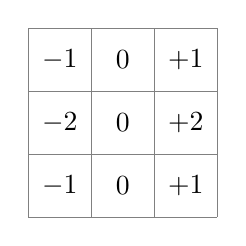
\begin{tikzpicture}
\draw[step=0.8cm,color=gray] (0,0) grid (2.4,2.4);
\node at (0.4,0.4) {$-1$};
\node at (1.2,0.4) {$0$};
\node at (2,0.4) {$+1$};
\node at (0.4,1.2) {$-2$};
\node at (1.2,1.2) {$0$};
\node at (2,1.2) {$+2$};
\node at (0.4,2) {$-1$};
\node at (1.2,2) {$0$};
\node at (2,2) {$+1$};
\end{tikzpicture}
\qquad
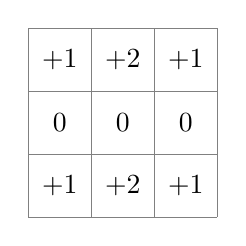
\begin{tikzpicture}
\draw[step=0.8cm,color=gray] (0,0) grid (2.4,2.4);
\node at (0.4,0.4) {$+1$};
\node at (1.2,0.4) {$+2$};
\node at (2,0.4) {$+1$};
\node at (0.4,1.2) {$0$};
\node at (1.2,1.2) {$0$};
\node at (2,1.2) {$0$};
\node at (0.4,2) {$+1$};
\node at (1.2,2) {$+2$};
\node at (2,2) {$+1$};
\end{tikzpicture}\hspace{\fill}\\\hspace{\fill}\\[-2ex]
\caption[Sobel Filters]{Sobel filters along horizontal axis (left) and vertical axis (right).}
\label{sobel}
\end{figure}
%Sobel Filters, which includes a weighted sum of neighboring pixels' gradients to approximate the gradient at the centering pixel
\noindent The image is then divided into small patches, and the magnitude and orientation of gradients within each patch are computed. After that, a histogram of gradients is computed, which contains 9 bins corresponding to angles 0, 20, 40 $\ldots$ 160. For each gradient, bins are selected based on its orientation, and the value that goes to the bins is based on the magnitude of the gradient. For instance, suppose a gradient has a magnitude of 3 and angle of 46 degrees. Since 46 is between 40 and 60, we select the two bins corresponding to 40 and 60 degrees. Now, since the difference between 46 and 40 is 6, and the difference between 46 and 60 is 14, the magnitude that goes to the bin corresponding to 40 degrees is $3 \times \frac{6}{20} = 0.9$, and the magnitude that goes to the bin corresponding to 60 degrees is $3 \times \frac{16}{20} = 2.4$. In this way, a histogram is computed to summarize the gradients within each patch.\\

\noindent Finally, we normalize the histograms and then concatenate them together to form a feature descriptor of the entire image. As indicated in figure \ref{visualization of HoG}, HoG serves as an edge detector of objects presented in an image \cite{7025824}.

\begin{figure}[h]
\captionsetup{justification=centering}
    \centering
    \includegraphics[scale=0.6]{images/hog_vis.png}
  % \centering
    \caption{Visualization of HoG.}
    \label{visualization of HoG}
\end{figure}

% \subsection{Graph Laplacian}

\section{Principal Component Analysis (PCA)}

Principal component analysis (PCA) is a commonly used dimensionality reduction technique in machine learning and statistics \cite{pca_reduction}. It attempts to find linear combinations of features in the original high dimensional data matrix to construct meaningful representation of the dataset \cite{doi:10.1080/14786440109462720}. 


\subsection{Definition}

\noindent 
Suppose the data consists of $n$ $m$-dimensional mean-centered examples $x^{(1)}, x^{(2)}, \ldots, x^{(n)}$ with $x^{(i)} \in \mathbb{R}^{m}$ $\forall i = 1,2, \ldots, n$. \\

\noindent
For any $k \in \{1,2, \ldots,  n\}$ and any set of orthonormal vectors $  u_1, u_2, \ldots, u_k \in  \mathbb{R}^{m}$, define the reconstruction error of the set of vectors as $$ \text{Err} (\{ u_1, u_2, \ldots, u_k\}) =  \sum_{i=1}^{n} || x^{(i)} - {  \hat{x}^{(i)}  }||_2^2$$ where $$\hat{x}^{(i)}   = \sum_{j=1}^{k} (u_i^{T} x^{(i)} )u_i  $$ is the projection of $x^{(i)} $ onto the subspace spanned by the given set of vectors.\\

\noindent The principle components (PCs) of the dataset are defined iteratively:

\noindent
The first PC $v_1$ is given by $$v_1 =  \text{argmin}_{||v||_2 =  1}  \text{Err} (\{v\}) $$

\noindent
For any $k \in \{1,2,\ldots, n-1\}$, after the first $k$ PCs $v_1, \ldots, v_k$ are determined, the $(k+1)^{th}$ PC is given by $$ v_{k+1} =  \text{argmin}_{||v||_2 =  1, v \perp v_i \; \forall i =1,2, \ldots, k}  \text{Err} (\{v_1, v_2, \ldots, v_k, v\}) $$


\subsection{Singular Value Decomposition (SVD)}
Formally, the SVD of a matrix $X \in \mathbb{R}^{n \times m}$ is a factorization of the form $X$ = $U \Sigma V^{T}$, where $U \in \mathbb{R}^{n \times n}, V \in \mathbb{R}^{m \times m}$ are orthonormal matrices, and $\Sigma \in \mathbb{R}^{n \times m}$ is a diagonal matrix consisting of non-negative entries.\\



\noindent SVD is often used to compute the principal components of a given dataset \cite{pca_via_svd}.  According to the following proposition, the principle components are exactly the right singular vectors of the matrix $X$, where $$X = [x^{(1)} \; x^{(2)} \ldots \; x^{(n)} ]^T$$
\noindent \begin{prop} \label{5.1}
Given any mean centered dataset $ x^{(1)}, x^{(2)}, \ldots, x^{(n)} \in \mathbb{R}^{m}$. The $k^{th}$ PC $v_k$ is the $k^{th}$ normalized right singular vector of $X$.
\end{prop}



\noindent The proposition allows us to efficiently compute the principle components of any given dataset using SVD algorithms. However, computing the exact value of SVD takes $O(mn \min (m,n))$ time, and the operations are not parallelizable. Therefore, it is not feasible when the values of $m$ and $n$ are large. Therefore, we also uses randomization techniques to trade accuracy for shorter run time:

\subsection{Randomized SVD}

\noindent Given any real matrix $X$ of dimension $n \times m$, the randomized power iteration SVD algorithm works as follows \cite{randomized_svd,random_svd2}:\\



        \noindent 1. Pick some small positive integers $k$, $p$, and $q$. Sample a matrix $\Omega$ of dimension $n \times (k+p)$, whose entries are IID standard normal.\\

 \noindent 2. Compute an SVD for $(XX^T)^{q}X\Omega  = Q DR$, and only keep the first $t$ columns of matrix $Q$, where $ t \leq k+p$ is the column rank of $D$.\\

 \noindent 3. Compute an SVD for $Q^T X = T \widetilde{ \Sigma} \widetilde{ V}^T$. Compute $\widetilde{U}= QT$, and return $\widetilde{ U} \widetilde{ \Sigma} \widetilde{ V}^T$ as an approximate SVD for $X$.\\
 
 
 


 \noindent Runtime of the algorithm is $O(mn \min (m,n))$, which is the same as that of the deterministic algorithm. However, since the most expensive operations in this algorithm are matrix multiplications, the algorithm can easily be parallelized, which results in a much shorter runtime. Furthermore, we can show that the expected approximation error of this algorithm approaches the optimal value as the value of $q$ increases:
 
 
\begin{theorem}Select a target rank $k \geq 2$ and an oversampling parameter $p \geq 2$. For any real matrix $X \in \mathbb{R}^{n \times m}$, select any integer $q \geq 0$ and execute the randomized power iteration SVD algorithm. Then
\begin{align*}
\mathbb { E } \left \| X - \widetilde{ U} \widetilde{\Sigma} \widetilde{V}^{T} \right\|_2 \leq \left [ \left( 1 + \sqrt { \frac { k } { p - 1 } } \right) \sigma _ { k + 1 }^{2q+1} + \frac { \mathrm { e } \sqrt { k + p } } { p } \left( \sum _ { j > k } \sigma _ { j } ^ { 2 (2q+1)} \right) ^ { 1 / 2 } \right ]^{\frac{1}{2q+1}}\tag{4.3} \label{Eq 4.3}
\end{align*}
\noindent where $\sigma_{j}$ is the $j^{th}$ singular value of $X$ $\forall j = 1,2, \ldots, n$.
\end{theorem}


\noindent If we bound the series in the inequality \ref{Eq 4.3} using its largest term $\sigma_{k+1}^{2(2q+1)}$ and draw the factor $\sigma_{k+1}$ out of the bracket, then
$$\mathbb { E } \left \| X - \widetilde{ U} \widetilde{\Sigma} \widetilde{V}^{T} \right\|_2 \leq \left[ 1 + \sqrt { \frac { k } { p - 1 } } + \frac { \mathrm { e } \sqrt { k + p } } { p } \cdot \sqrt { \min \{ m , n \} - k } \right] ^ { 1 / ( 2 q + 1 ) } \sigma _ { k + 1 }$$

\noindent
As $q$ becomes larger, the expression on the right approaches $ \sigma_{k+1}$, which is the smallest possible approximation error for any rank-$  k $ matrix.\\


\noindent In conclusion, the randomized SVD algorithm enables us to compute a close approximation of the singular value decomposition for any real matrix within a relatively short amount of time. Hence we use this algorithm to reduce the dimensionality of our data.

 
 
 
\section{Pixel-wise Anomaly Measure}

\noindent Given an image, we approximate the distribution of red, green, and blue intensities, and then assign each individual pixel an anomaly score based on how much the pixel's intensity deviates from the estimated global distribution \cite{RX_detector}. This process can be done using graph-based method described below \cite{graph_lap} as follows.\\

\noindent Consider an undirected, weighted graph $G = (V,E)$ composed of a vertex set $V =\{r,g,b\}$ corresponding to the three color intensities, and an edge set $E$ specified by $(a, b, w_{ab})$, where $a, b \in V$, and $w_{ab} \in \mathbb{R}^{+}$ is the edge weight between vertices $a$ and $b$.  In our case, the edge weights are defined as:
\begin{align}
w_{rg}=\frac{1}{1+\left(\frac{\mu_{r}-\mu_{g}}{\alpha}\right)^{2}}, w_{rb}=\frac{1}{1+\left(\frac{\mu_{r}-\mu_{b}}{\alpha}\right)^{2}}, w_{gb}=\frac{1}{1+\left(\frac{\mu_{g}-\mu_{b}}{\alpha}\right)^{2}}
\end{align}
\noindent where $\alpha = \frac{\mu_a + \mu_g + \mu_b}{3}$ and $\mu_r, \mu_g, \mu_b$ are the average red, green, and blue intensities in the image, respectively. From the adjacency matrix $W$, the combinatorial graph Laplacian matrix
$L = D - W$ can be computed, where $D$ is the degree matrix defined by:
\begin{align}
D(a, b)=\left\{\begin{array}{ll}{\sum_{k=1}^{n} w_{a k}} & {\text { if } a=b} \\ {0} & {\text { otherwise }}\end{array}\right.
\end{align}\hspace{\fill}\\
\noindent Finally, we normalize the Laplacian matrix $
L^{*}=D^{-\frac{1}{2}}L D^{-\frac{1}{2}}
$ and define an anomaly measure for each pixel $x$ in the image by:
$$ \delta(x) = s^T L^* s,$$
 \noindent where $s \in \mathbb{R}^3$ is the color intensity of $x$.\\





\noindent The anomaly measures can be used to identify anomalous pixels as shown in the figures below:

\begin{figure}[H]
    \centering
    \includegraphics[scale=0.5]{images/graph_laplacian_1.png}
    
    
    \includegraphics[scale=0.5]{images/graph_laplacian_2.png}
  % \centering
    \caption{Results of the graph-based anomaly detection algorithm.}
    \label{fig:graphlaplacian}
\end{figure}



\noindent The images on the left are examples with artifacts. The binary images on the right are the results of the graph-based anomaly detection algorithm, where pixels in white have anomaly measure exceeding the mean value by at least two standard deviations. As we can see from the figures, most pixelated patches and discolorated pixels have high anomaly scores. \\

\noindent Since corrupted pixels tend to appear together in clusters, we apply dilation to the results of the anomaly detection algorithm to fill in small holes in each cluster \cite{dilation}. Here dilation refers to setting any pixel in a binary image to 1 if any of its neighboring pixels have the value 1. An example is shown in Figure \ref{fig:dilation}.


\begin{figure}[H]
    \centering
    \includegraphics[scale=0.5]{images/dilation.png}
    
    
  % \centering
    \caption{Applying dilation to the results of the graph-based anomaly detection algorithm.}
    \label{fig:dilation}
\end{figure}



\noindent However, sometimes pixels with high anomaly scores are not corrupted, as shown in the figure below. Therefore we combine pixel-wise anomaly measure with other features in order to detect artifacts without producing too many false positives.

\begin{figure}[H]
    \centering
    \includegraphics[scale=0.5]{images/graph_laplacian_false_postive.png}
    

  % \centering
    \caption{False positives produced by the graph-based anomaly detection algorithm.}
    \label{fig:graphlaplacianfp}
\end{figure}



\noindent 

\endinput

% % Chapter 4
\ifthenelse{\boolean{@twoside}}{\myclearpage}{}
\chapter{Artifact Classification}\label{Ch:classification}


In order to classify the artifacts we considered a variety of machine learning algorithms, under both supervised and unsupervised categories. Supervised learning algorithms use labeled data to learn how to classify the data based on the given labels (categories), while unsupervised models infer patterns in the data without referring to the labels. Here we discuss the different algorithms that we tried in order to perform a binary classification (corrupted vs. normal) on our data.

\section{Classical Machine Learning Methods}\label{classic}
In order to train supervised algorithms, we need labeled data. In other words, for each training instance, we need to know whether it is corrupted and what type of artifact it contains. Since we have collected normal images and produced corrupted images, we are ready to train supervised learning algorithms:

\subsection{Linear Discriminant Analysis (LDA)}

In our study, we have used the two-class linear discriminant analysis (LDA) \cite{scikit-learn} as one of the individual artifact detection models. Consider the set of features $\Vec{x}$ for each sample and its associated label $y$. To predict class labels given a specific set of features $\Vec{x}$, we look at the log-likelihood ratio,
$$ \log\left( \frac{P(y=0 | \Vec{x})}{P(y=1 | \Vec{x})} \right) = \log\left( \frac{P(\Vec{x}| y = 0) P(y = 0)}{P(\Vec{x}| y = 1) P(y = 1)} \right)$$
LDA assumes that the conditional probability density functions $P(\Vec{x} | y = 0)$ and  $P(\Vec{x} | y = 1)$ are both normally distributed with mean and covariance $(\Vec{\mu_0}, \Sigma_0)$ and $(\Vec{\mu_1}, \Sigma_1)$, estimated from the training data. Also, we can estimate $P( y = 0)$ and $P( y = 1)$ by the proportion of samples from class $0$ or $1$. In the LDA case, we further assume that the Gaussian distributions for each class share the same covariance matrix, so $\Sigma_0 = \Sigma_1 = \Sigma$. Using the multivariate Gaussian assumption, we will predict class label 0 if:

\begin{equation*}
\begin{split}
    & \log\left( \frac{P(y=0 | \Vec{x})}{P(y=1 | \Vec{x})} \right)  > 0 \\
    \iff & \log\left( \frac{P(\Vec{x}| y = 0) P(y = 0)}{P(\Vec{x}| y = 1) P(y = 1)} \right) > 0 \\
    \iff & (\Vec{\mu_0} - \Vec{\mu_1})^t \Sigma ^{-1} \Vec{x} > \frac{1}{2} (\Vec{\mu_0}^{t} \Sigma^{-1} \Vec{\mu_0} - \Vec{\mu_1}^{t} \Sigma^{-1} \Vec{\mu_1} ) -\log \frac{P(y=0)}{P(y=1)}
\end{split}    
\end{equation*}



\subsection{Support Vector Machine (SVM)}

Consider the case where there are two classes of data (blue and green) that are linearly separable:

\begin{figure}[H]
    \centering
    \includegraphics[scale=2.0]{images/svm.png}
  % \centering
    \caption{2-D Linearly Separable Data.}
    \label{ls-svm}
\end{figure}

\noindent Support vector machine compute the decision boundary that maximizes the margin, which is defined as the distance of the closest data point to the decision boundary \cite{Cortes95support-vectornetworks}. Mathematically, support vector machine is a function $f: \mathbb{R}^m \rightarrow \{1,-1\}$, where $m$ is the dimension of the data, and $1$ and $-1$ correspond to the two classes. Suppose the number of data is $n$, then the function $f$ is given by:
$$\Scale[1.2]{f(x) = \text{sign} (\mathbf{w}\mathbf{x}+\mathbf{b})}$$ where $\mathbf{w}$ and $\textbf{b}$ are solutions to the following optimization problem:
$$\Scale[1.2]{\begin{array}{ll}{\min _{\mathbf{w}, b}} & {\frac{1}{2} \mathbf{w}^{\top} \mathbf{w}} \\ {\text { s.t. }} & {y_{i}\left(\mathbf{w}^{\top} \mathbf{x}_{i}+b\right) \geq 1, \quad i=1, \ldots, n }\end{array}} $$

\noindent The optimization problem is typically solved via its dual problem. In the case where the data is not linearly separable, there is no solution to the optimization problem above. Therefore we add slack variables $\xi_i \; \forall i = 1,2, \ldots, n$ to the problem, which allows data points to be within the margin \cite{soft_svm}:
$$\Scale[1.2]{\begin{array}{c}{\min _{w, b, \xi \geq 0} \frac{1}{2} \mathbf{w}^{\top} \mathbf{w}+C \sum_{i} \xi_{i}} \\ {\text { s.t. } y_{i}\left(\mathbf{w}^{\top} \mathbf{x}_{i}+b\right) \geq 1-\xi_{i}, \quad i=1, \ldots, n}\end{array}}$$

\noindent The SVM algorithm can be generalized to classify more than two classes. There are also many other supervised learning algorithms such as random forest and convolutional neural network that can be applied to identify corrupted images. We expect them to perform well in identifying known artifacts. On the other hand, supervised algorithms will probably not able to detect unknown artifacts. As a result, we also consider applying unsupervised algorithms.


\subsection{Logistic Regression}
One of the most commonly used statistical tools for binary classification is logistic regression which is an extension to linear regression. As opposed to linear regression which fits a straight line or a hyperplane to the data, logistic regression uses the logistic function to squeeze the output of a linear equation between 0 and 1, thereby producing a probability \cite{logistic}. The logistic function is defined the following:

\begin{equation}
\operatorname{logistic}(\eta)=\frac{1}{1+\exp (-\eta)}
\label{logistic}
\end{equation}

\begin{figure}[H]
    \centering
    \includegraphics[scale=0.3]{images/log.png}
    \caption[Logistic Function]{Logistic (sigmoid) function maps the input to a number between 0 and 1.}
    \label{log}
\end{figure}

\noindent
Similar to linear regression where the model learns the weights $\beta_i$ that minimize the prediction error (illustrated in Equation \eqref{linear}), logistic regression minimizes the loss function, with the linear model given as input to the logistic function in order to produce a number between 0 and 1 (see Equation \eqref{log_eq}). Gradient decent is used to find the minimum of the loss function.


\begin{equation}
\hat{y}^{(i)}=\beta_{0}+\beta_{1} x_{1}^{(i)}+\ldots+\beta_{p} x_{p}^{(i)}
\label{linear}
\end{equation}

\begin{equation}
P\left(y^{(i)}=1\right)=\frac{1}{1+\exp \left(-\left(\beta_{0}+\beta_{1} x_{1}^{(i)}+\ldots+\beta_{p} x_{p}^{(i)}\right)\right)}
\label{log_eq}
\end{equation}


%%%%%%%%%%%%%%%%%%%%
\newpage
%%%%%%%%%%%%%%%%%%%%

\section{Deep Learning Methods}\label{deep}

\subsection{Convolutional Neural Network}

\noindent Convolutional Neural Network (CNN) is a class of deep neural networks which are often applied to analyzing visual imagery \cite{cnn_anomaly1}\cite{cnn_anomaly2}. Compared to other image classification algorithms, CNN requires relatively little pre-processing since it is able to automatically extract features from the training data.\\

\noindent A convolutional neural network consists of several types of layers, including fully connected layer, convolutional layer, and pooling layer \cite{cnn}. In a fully connected layer, each neuron is connected to every neuron in the previous layer. In a convolutional layer, however, each neuron is connected to a restricted subarea of the previous layer. Pixels within the subarea are convolved with a filter whose parameters are learned during the training step, and the result is passed to the corresponding neuron in the convolutional layer. Moreover, pooling layers reduce the dimensions of the data by combining the values in a subarea in the previous layer into a single neuron in the pooling layer. For instance, max pooling uses the maximum value within each subarea, and average pooling uses the average value within each subarea.\\

\begin{figure}[h]
\captionsetup{}
\includegraphics[scale=0.5]{images/cnn_structure.png}
\caption[Structure of our CNN model]{Structure of our CNN model. There are 5 convolutional layers, each followed by a max pooling layer. The two layers before the final output layers are fully connected.}
\label{fig:cnnstructure}
\end{figure}


\noindent Similar to other deep learning models, CNN is trained using back-propagation. We choose cross-entropy \cite{loss_function} as the loss function for our model, which is defined by:
$$ g(x) = - l_t (x) \log l_p (x) - (1-l_t (x)) \log (1 - l_p(x))$$

\noindent where $l_t(x) \in \{0,1\}$ is the true label of instance $x$ and $l_p(x) \in \{0,1\}$ is the predicted label of instance $x$ (here normal class corresponds to label 0, and corrupted class corresponds to label 1). The parameters of the model are updated through gradient descent in order to minimize the loss function. During testing, each instance is fed into the CNN, and the model outputs the probability that the instance is corrupted.\\

\subsection{Generative Adversarial Network}

\noindent Generative Adversarial Network has been a popular area of research in deep learning during recent years. We consider to apply GAN to detect artifacts because it only requires normal images as training data. GAN consists of two components: a generator $G$ and a discriminator $D$. The generator is supposed to take in random noise and generate fake images that resemble training data, and the discriminator is supposed to distinguish images produced by the generator from the training data \cite{gan}. \\


\begin{figure}[h]
\centering
\includegraphics[scale=0.3]{images/gan.png}
\caption{Structure of a GAN.}
\label{fig:structureGAN}
\end{figure}

\noindent The model's loss function is defined by:

$$
\min _{G} \max _{D} V(D, G)=\mathbb{E}_{\boldsymbol{x} \sim p_{\text {data }}(\boldsymbol{x})}[\log D(\boldsymbol{x})]+\mathbb{E}_{\boldsymbol{z} \sim p_{\boldsymbol{z}}}(\boldsymbol{z})[\log (1-D(G(\boldsymbol{z})))]
$$

\noindent The two components in a GAN are trained an iterative numerical approach. When training the discriminator $D$, the parameters in the generator, $\theta^{(D)}$, are held fixed, and the parameters in $G$, $\theta^{(G)}$, are updated using gradient ascent to maximize the loss function:

$$\theta^{(D)} \leftarrow \underset{\theta^{(D)}}{\arg \max }\left[ \mathbb{E}_{x \sim p_{\text {data }}} \log D(\mathbf{x})+ \mathbb{E}_{\mathbf{z}} \log (1-D(G(\mathbf{z})))\right]$$

\noindent When training the generator, $\theta_D$ are held fixed, and $\theta_G$ are updated using gradient descent to minimize the loss function:

$$\theta^{(G)} \leftarrow \underset{\theta^{(G)}}{\arg \min }  \mathbb{E}_{\mathbf{z}} \log (1-D(G(\mathbf{z})))$$

\noindent It can be shown that a unique global optimal solution exists, where the generator learns the distribution of the training data and the discriminator outputs the probability of the input image being real as $\frac{1}{2}$ all the time, which indicates that it is not able to distinguish fake images produced by the generator from the training data.\\


\noindent Most research done on GAN focuses on the generator \cite{style_gan}. However, we think the discriminator may be able to identify anomalous images that are different from the training data. Therefore we use a generative adversarial model that are trained on normal data to detect artifacts.
%%%%%%%%%%%%%%%%%%%%
\newpage
%%%%%%%%%%%%%%%%%%
\section{Ensemble Methods}
Initially, we approached the classification stage by training a single CNN model that would discriminate between corrupted images (regardless of the artifact type) from normal. However, the unsatisfactory performance suggested that a single model might be unable to capture cross-class patterns in the scope of this project. Thus, we switched to a mixed experts ``ensemble'' model that combines multiple learning algorithms, each of which specializes in identifying one particular artifact type. Our classification procedures can thus be described as follows.

\begin{enumerate}
    \item \textbf{Training Stage 1.} First, we trained the individual models for binary classification for each corruption type. For this training procedure, we extracted images from 24 games (dataset $A$ in Table \ref{games}), kept 2,400 of those images as normal and applied \texttt{Glitchify} to the rest, obtaining around 1,500 frames per corruption type. A variety of models introduced in Sections \ref{classic} and \ref{deep} were paired with features from Chapter \ref{Ch:feature} and trained as binary classifiers for each artifact type from Chapter \ref{Ch:datagen}. The best models were then selected and their performances were recorded in Table \ref{tab:models}. Table \ref{fig:methods-tried} shows all pairings ``artifact-feature-model'' that were considered in the scope of this project.
    
    \item \textbf{Training Stage 2:} after putting together the individual trained models, we train a logistic regression on the output of the individual models concatenated together. At this stage, our dataset comprised of 3 games (dataset $B$ in Table \ref{games}) - never seen by the individual models - with 1650 normal images and 150 images of each type of artifact. A 0.25/0.75 test-train split was applied to the data. At this stage, all of the models are given normal images in addition to all types of artifacts. The performance on the test set is reported in Table \ref{tab:stage2}.
    \item \textbf{Testing:} the goal of this stage is to measure the generalizability of the ensemble model. That is, how well the ensemble performs on games it has never seen before. The heldout test set was composed of 3 games (see dataset C in Table \ref{games}), with 1650 normal images and 1800 corrupted images, which is 150 for each artifact type. All of these images were used to test the ensemble. The results are reported in Tables \ref{tab:variation} and \ref{tab:test_models}.
\end{enumerate}

\newpage

\begin{figure}[!h]
  \centering
  \includegraphics[scale=0.3]{images/stage_1.png}
  \caption*{Training Stage 1.}
  \centering
  \includegraphics[scale=0.4]{images/stage2.png}
  \caption*{Training Stage 2.}
\caption[Ensemble Model]{The Architecture of the Ensemble Model. The input consists of $N$ observations with $M$ features. The ensemble produces a binary output of ``normal" or ``corrupted''. }
\label{fig:ensemble}
\end{figure}

\noindent 
Given the scope of this project, we were not able to apply all possible feature extraction and modeling combinations to all of the artifacts. Therefore, for each artifact, we thought about which feature representations can capture that artifact the best, and we only applied those methods. For example, there are no repetitive patterns in screen tearing artifacts so we did not consider using Fourier transform to extract features. Figure \ref{fig:methods-tried} illustrates what models we considered for each artifact.

\begin{figure}[!h]
  \centering
  \includegraphics[scale=0.3]{images/results-methods.png}
  \caption{Methods we tried for each artifact.}
\label{fig:methods-tried}
\end{figure}


% \begin{comment}
% \begin{table}[!ht]
% \centering
% \begin{tabular}{@{}lllll@{}}
% \toprule
% Feature & Classification Model & Corruption Type  \\ \midrule
% Resized Image & 580 & 1070\\
% Resized FT (magnitudes) & 1241 & 409\\
% Resized FT (magnitudes) \& PCA & 832 & 818\\
% Image Statistics & 1641 & 9\\
% Histogram of Gradients & 1621 & 29\\\bottomrule
% \end{tabular}
% \caption[Individual model combinations]{Individual classifiers considered (selected combinations shown in bold).}
% \label{fig:methods-tried}
% \end{table}
% \end{comment}

\noindent 
We considered two input formats for the ensemble model---binary outputs of the individual classifiers and their raw probability vectors. In addition, we attempted to employ an $OR$ logic concatenation of the individual models, however, this yielded poor performance due to the cumulative effect of false positive rates of the individual models.\\

\noindent 
In addition to the ensemble structure explained earlier - in which the individual models have a binary output of 0 or 1 and a logistic regression is trained on those outputs - we considered a number of different approaches.
\begin{enumerate}
    \item\textit{Probabilities output of individual models}. n this case, instead of having each of the individual models output 1 or 0, we had them output a probability, and trained the logistic regression on those probability vectors (still in $\mathbb{R}^{10}$). If a model was not equipped with a probability output (i.e SVM) we just used the binary output.
    \item\textit{Using OR logic}. Instead of using a logistic regression to produce binary outputs for the ensemble model, we could also use the or logic. This means that for a given image, if at least one model flags it as ``corrupted", then the ensemble will flag that image as corrupted. In other words if the magnitude of $z^i$ in Figure \ref{fig:ensemble} is greater than 0, then the ensemble will flag the $i^{th}$ image as ``corrupted".
\end{enumerate}

\section{Performance Metrics}
In order to evaluate the performance of our models, we have adopted three different metrics: accuracy, precision and recall. Let an image that is predicted to contain glitches be ``positive" and an image that is predicted to be normal be ``negative." Then, if a glitched image is labeled as ``glitched" correctly, it is a true positive (TP); otherwise, it is a false negative (FN) if our model mislabels it as a normal image. Similarly, if a normal image is labeled as ``normal" correctly, it is a true negative (TN); otherwise, it is a false positive (FP) if our model mislabels it as glitched. The definitions of the three metrics are as follows:
\begin{align}
\text{Accuracy}&=\frac{\text{TP+TN}}{\text{TP+FP+TN+FN}},\\\nonumber
\text{Precision}&=\frac{\text{TP}}{\text{TP+FP}},\\\nonumber
\text{Recall}&=\frac{\text{TP}}{\text{TP+FN}}\nonumber.
\end{align}
\noindent In the next section, we will present the results of our classification models. The model performances are evaluated in terms of accuracy, precision and recall as defined above.

\endinput

% Chapter 5
\ifthenelse{\boolean{@twoside}}{\myclearpage}{} 
\chapter{Results}\label{Ch:results}




In this section we will cover the main classification results, as well as some results that were obtained by looking at a subset of artifacts.
\section{Performance of CNN}
Even though CNNs are widely used for computer vision and object detection, we did not find them to be useful for artifact detection. The performance of CNN on three artifacts in in Table \ref{tab:cnn}. The reason we are not showing other artifacts in this table is that the CNN was not able to train on those artifacts (the loss function either got stuck in a local minimum or never converged). It must be noted that we did not spend much time on hyper parameter tuning, therefore better results could be reached by using other hyper parameters.

\begin{table}[h]
    \centering
    \includegraphics[scale=0.4]{images/CNN.png}
    \caption{Performance of Convolutional Neural Network  on Three Artifacts.}
    \label{tab:cnn}
\end{table}

\section{Performance of the ensemble on familiar games}
In training stage 1 and training stage 2, 25\% of the data (from data set A and data set B, respectively) was held out as test set. This means that when evaluating the models on these test sets, 1. the individual models have already seen the games in test set taken from data set A, and 2. the logistic regression has already seen (other images from) the games that were used in the test set taken from data set B. Table \ref{tab:models} and Figure \ref{fig:stage1} show the results of testing the individual models (after training stage 1). At this stage, the models are performing on familiar games. That is, the models have seen different images from the same games during training.\\

\noindent
As for the logistic regression, Table \ref{tab:stage2} contains the results of training the logistic regression (training stage 2 trained on data set B). We set aside 25\% of the data set B to test the performance of logistic regression on familiar games which turned out to have an accuracy of 84\%.
\begin{table}[h]
    \centering
    \includegraphics[scale=0.8]{tables/models.pdf}
    \caption{Performance of models in training stage 1.}
    \label{tab:models}
\end{table}

%\begin{landscape}
%\centering
%\begin{table}
%    \centering
%    \includegraphics[scale=0.8]{tables/stage2.pdf}\\[-15ex]
%    \caption{Performance of models in training stage 2.}
%    \label{tab:stage2}
%\end{table}
%\end{landscape}

\begin{table}
\centering
\begin{tabular}{@{}lllll@{}}
\toprule
Model (Artifact) & Testing Time (min) & Accuracy & Precision & Recall  \\ \midrule
Shapes & 19 & 0.49 & 0.07 & 0.81\\
Line pixelation & 7.4 & 0.91 & 0.33 & 0.91\\
Shader & 2.8 & 0.54 & 0.08 & 0.91\\
Morse code & 9.5 & 0.98 & 0.66 & 1.00\\
Parallel lines & 6.9 & 0.98 & 0.67 & 0.99\\
Dotted line & 6.9 & 0.71 & 0.12 & 0.85\\
Stuttering & 6.9 & 0.90 & 0.31 & 0.94\\
Triangulation & 6.9 & 1.00 & 1.00 & 1.00\\
Discoloration & 6.9 & 0.76 & 0.15 & 0.95\\
Screen tearing & 2.8 & 0.67 & 0.02 & 0.11\\
\midrule
\bf{Random Forest} & \bf{N/A} & \bf{0.71} & \bf{0.79} & \bf{0.56}\\
\bf{Logistic Regression} & \bf{N/A} & \bf{0.84} & \bf{0.9} & \bf{0.77}\\\bottomrule
\end{tabular}
\caption{Performance of models after training stage 2.}
\label{tab:stage2}
\end{table}

\section{Performance of the ensemble on new games}
\noindent An important metric in assessing artifact detection models is generalizability. In our case, generalizability refers to the ability of the model to perform equally well when images come from games unseen during training. We can measure not only the generalizability of the final logistic regression, but also that of individual models. \\

\noindent
Recall that in training stage 2, even though the logistic regression has seen the games in dataset B, the individual models have not. Therefore the performance of the individual models in Table \ref{tab:stage2} is a measure of their generalizability to new games. Figure \ref{fig:stage2} is a visualization of the models in Table \ref{tab:stage2}. \\
 
\noindent
We also tested the generalizability of the ensemble model. For this purpose, we tested it on data set $C$ which it has never seen before, and obtained an accuracy of 69\%. The second row of \ref{tab:variation} contains other metrics on the performance of the logistic regression on the heldout test set. The performance metrics of the individual models on this test set is restricted to True Negative and False Positive (Table \ref{tab:test_models}). This is because our test data was labeled as 0 or 1, and therefore we cannot tell how many false negatives and true positives of a given model are the specific artifact type of the model, or other artifacts. \\

%maybe this should go to the Discussion chapter
\noindent The difference in performance of models in Table \ref{tab:models}
and Table \ref{tab:stage2} is that in Table \ref{tab:models}, not only are the individual models tested on games that they have seen before, but also they are tested on a dataset that only consists of normal images and the corrupted images that each model is trained to detect. In Table \ref{tab:stage2} the models are tested on images coming from games that they have never seen, in addition to corruptions they have never seen. In Table \ref{tab:stage2} we can see that the Shapes and Shader models have low accuracy of 0.49 and 0.54 respectively. Therefore we conduct an experiment where we excluded these two models while keeping the artifacts in the data (Table \ref{tab:variation}). Additionally we retrained the logistic regression after excluding the screen tearing model and artifact from the data. We also trained the logistic regression on probability outputs instead of binary outputs. The results are shown in Table \ref{tab:variation} and Figure \ref{fig:probability}.


\begin{figure}
    \centering
    \includegraphics[scale=0.7]{images/stage1fig.pdf}
    \caption[Performance of models in training stage 1]{Performance of models in training stage 1. The models are tested on games they have seen before.}
    \label{fig:stage1}
\end{figure}


\begin{figure}
    \centering
    \includegraphics[scale=0.7]{images/stage2fig.pdf}
    \caption[Performance of models in training stage 2]{Performance of models in training stage 2. The models are tested on new games.}
    \label{fig:stage2}
\end{figure}


%\begin{table}
%    \centering
%    \includegraphics[scale=0.6]{tables/test_models.png}
%    \caption{Performance of models on the heldout test set.}
%    \label{tab:test_models}
%\end{table}

\begin{table}
\centering
\begin{tabular}{@{}lllll@{}}
\toprule
Model (Artifact) & True Negative & False Positive  \\ \midrule
Shapes & 580 & 1070\\
Line pixelation & 1241 & 409\\
Shader & 832 & 818\\
Morse code & 1641 & 9\\
Parallel lines & 1621 & 29\\
Dotted line & 1455 & 195\\
Stuttering & 1301 & 349\\
Triangulation & 1650 & 0\\
Discoloration & 1571 & 79\\
Screen tearing & 1467 & 183\\\bottomrule
\end{tabular}
\caption{Performance of models on the heldout test set.}
\label{tab:test_models}
\end{table}

%\begin{table}
%    \centering
%    \includegraphics[scale=0.5]{tables/variation.png}
%    \caption{Performance of variations of LR.}
%    \label{tab:variation}
%\end{table}

\begin{table}
\centering
\begin{tabular}{@{}lllll@{}}
\toprule
Model & Accuracy & Precision & Recall  \\ \midrule
LR (full, seen games, binary) & 0.84 & 0.90 & 0.77\\
LR (full, unseen games, binary)& 0.69 & 0.67 & 0.82\\
LR (no screen tearing, unseen games, binary) & 0.70 & 0.68 & 0.79\\
LR (no shapes/shader, unseen games, binary) & 0.68 & 0.66 & 0.82\\
LR (full, unseen games, probability) & 0.66 & 0.60 &  0.90\\\bottomrule
\end{tabular}
\caption{Performance of variations of LR.}
\label{tab:variation}
\end{table}

\begin{figure}
    \centering
    \includegraphics[scale=0.7]{images/probability.pdf}
    \caption[Performance of logistic regression on probability output]{The performance of the Logistic Regression trained on binary vs. probability output of the individual models.}
    \label{fig:probability}
\end{figure}




\section{Comparison to AMD's model}
AMD was able to run their model on our heldout test set (Data set C). In Figure \ref{fig:comparison} we can see that our models have similar accuracy, however, our model was able to achieve a higher recall score of 0.82 compared to AMD's score of 0.71.

\begin{figure}
    \centering
    \includegraphics[scale=0.7]{images/comparison.pdf}
    \caption{Comparison of AMD's model and ours}
    \label{fig:comparison}
\end{figure}
\endinput


% Chapter 6
\ifthenelse{\boolean{@twoside}}{\myclearpage}{}
\chapter{Discussion, Conclusion and Future Work}\label{Ch:discussion}

\section{Discussion}
We now discuss possible interpretations of our results as well as their limitations and sources of possible bias. One fundamental concern relates to our own ``synthetic'' dataset and its representation of the actual graphics corruptions that occur during gameplay. First, our approach in developing the \texttt{Glitchify} program consisted of classifying artifacts into categories based on their appearance, however, the viability of this procedure is debatable. Whereas the structure and design of screen-tearing and stuttering were sufficiently understood and formally expressed, our definition of shader/shapes and line pixelation artifacts might be too narrow to capture all of the variations of these corruptions seen in reality. This discrepancy might be responsible for some bias present in our artificial dataset, which in turn affects all further results.\\\hspace{\fill}\\
Another data-related concern comes from the frames we extracted from games to feed into \texttt{Glitchify}. We require that all these frames are normal, i.e. do no contain any corruptions. In order to ensure this holds, we manually processed collected images in an attempt to perform a first-order quality check. Due to surrealistic contents of most games, working with individual frames rather that a continuous gameplay makes it harder, if not impossible, to correctly discriminate between unwanted artifacts and intentional design. Figure \ref{confused} displays examples of such images.
\begin{figure}[H]
\centering
\includegraphics[scale=0.18]{images/corr2.png}
\includegraphics[scale=0.16]{images/shape3.jpg}\\[2ex]
\caption{A normal (left) and a corrupted (right) images.}
\label{confused}
\end{figure}

%%%%%%%%%%%%%%%%%%%%
\newpage
%%%%%%%%%%%%%%%%%%%%%
\noindent
Regarding the individual models, the accuracy on the test set drops from training stage 1 (Table \ref{tab:models}) to training stage 2 (Table \ref{tab:stage2}). This is mostly due to the fact the models in training stage 2 have never seen the games they are being tested on. In this project, however, the recall rate is the most important metric to consider as it is crucial to make sure that during gameplay, we detect as my corrupted images as possible so we can fix them. In training stage 2, we can see that most models produce good recalls on games they have never seen, showing a good degree of generalizability. The artifacts comprising Discoloration and Screen Tearing have very low recall scores in training stage 2 (0.66 and 0.5 respectively) versus 0.95 and 0.80 in training stage 1, demonstrating that those models overfit the training data and are not generalizable to new games. We speculate that the low accuracy score we have obtained on the heldout test set is due to the ``glitchy" look of one of the games we have included in data set C (Crackdown 3). Both images in Figure \ref{fig:hard} are from this game. Additionally, there are a lot of explosions that happened during the gameplay, and we suspect that the frames we labeled as ``normal" are not entirely normal.\\

\begin{figure}[h]
    \centering
    \includegraphics[scale=0.11]{images/discoloration_146.jpg}
    \includegraphics[scale=0.11]{images/dotted_line_345.jpg}
    \includegraphics[scale=0.11]{images/shader_1.jpg}
    \includegraphics[scale=0.11]{images/screen_tearing_132.jpg}
    \includegraphics[scale=0.11]{images/shape_56.jpg}
    \includegraphics[scale=0.11]{images/shape_91.jpg}
    \caption[Visualization of False Positives]{Visualization of False Positives. On the left, from top to bottom the normal images are misclassified as discoloration, shader, shape. On the right, from top to bottom the images are misclassified as dotted line, screen tearing, shape.}
    \label{fig:FP}
\end{figure}



\noindent Another metric that we consider which is less important than recall is precision. Precision is the ratio of corrupted images over the images that were predicted to be corrupted. A low precision corresponds to a high number of false positives. In Table \ref{tab:stage2}, we can see that most models produce a large number of false positives. This means that these models are conservative and label a lot of normal images as corrupted. After looking at Figure \ref{fig:FP} we can see that some games truly look like they have an artifact, and until the models see those games and learn what is ``normal", it is expected for them to produce a lot of false positives.\\

%\noindent There are some limitations and biases associated with how we conducted the data generation. First and foremost, the images we extracted from videos may have already contained artifacts (i.e texture pop-in) due to compression. Also, some frames may look ``glitchy” but they are actually not. Examples of this are in Figure \ref{fig:FP} where models missclassified normal images as corrupted. We did go through the images manually to make sure that they do not already contain glitches, but did not perform the manual vetting exhaustively over the whole dataset. \\

%\noindent Second, when extracting images from gameplays on YouTube\texttrademark, even though some videos covered the entire gameplay, a number of them only covered one or a few chapters of the game. This means that not all environments/states in that game were represented which restricts the scope of our data. This could potentially lead to our model being less robust. Additionally, screen tearing artifacts that are produced from static games can be very hard to detect, if not impossible. This leads to inaccurate labels which make it difficult for the model to converge. \\ 

%\noindent Another source of bias in our data is the pace of the game. If the game is dynamic (i.e action adventure games) where the scene is constantly changing, then sampling frames at even a high rate will result in images that are independent. On the other hand, if the game is slowly changing (i.e strategy games), then sampled frames can look very similar. This could introduce large amounts of bias in the results of the model if the images in the test set are close to those in the training set. Another existing limitation is the fact that we resize the images before feeding them to most  models. By resizing the images we lose some potentially useful information which can also reduce the strength of the rendered artifacts. 
\noindent
\\
\\
\noindent
Finally, the challenge is to find models that best perform the task of classification. Due to time limits, we were unable to try all the deep-learning models due to the long training time the tedious fine tuning that they require. Nevertheless, we have found that some traditional machine learning models that are frequently used as classifiers and take less time to train - such as logistic regression- can handle the artifact detection task well. Using the dimension-reduced features of the images as inputs, we constructed a number of machine learning models as individual glitch classifiers and selected the best models with the highest accuracy for each glitch. Our ensemble model combined all the best individual classifiers, but some models which had relatively poor performance (for example, the model used to detect little square patches) caused a lot of false positives and negatives. Since the square patch glitches were not always visible to humans, we have excluded those images with square patches from both the training sets and the testing sets. Yet the detection of the less obvious glitches might still be worth thinking about in the future.



\section{Conclusion}
In this study, we developed a software that automatically detects graphics corruptions in frames from video games. Based on a sample of screen corruption examples provided by AMD, 13 most common content-unrelated artifacts were selected, described and then recreated with a \texttt{Glitchify} program. With help of \texttt{Glitchify}, a dataset of 50,000 images was created by adding 13 different types of artifacts to normal frames extracted from 34 modern video games. Each of the 13 corruptions was learned by different models including Logistic Regression, Support Vector Machine and Linear Discriminant Analysis. The output probabilities of these individual classifiers were used for training a mixed experts Logistic Regression model intended to carry out the final classification decision. The overall accuracy on the \texttt{Glitchify}-produced test set based on games unseen during training is 69\%. 


\section{Future Work}
One promising way we can improve our results is tiling. That is, instead of resizing the images which could lead to loss of information, we break the image down into ``tiles" and treat each tile as a single image. This would require us to have knowledge about where in the image the artifacts have been inserted, so we can label the tiles appropriately. Although tiling might lead to loss of context, it could still improve our performance since we are not resizing the images.\\
Another possibility in improving our work is to conduct a finer hyper parameter grid search to train our CNN.\\

% In the future, we would like to train our model on more images, and include more games in our testing set to better evaluate the generalizability of our models. Also, we may explore more ways to represent the features and more machine-learning approaches to do the classification task. A finer grid-search of the hyper-parameters of some models can also be done to improve the performance of the models. Finally, we could search for other methods to better combine the results from individual classifiers and improve the ensemble model. \\
\noindent Since our model currently only focuses on binary classification (glitched or normal), building a multi-class classifier which outputs the type of the detected glitch would be very ideal. Since the ensemble is composed of individual models each of which are capable to detecting a specific type of glitch, the multi-class classification is feasible. \\

\noindent Another future direction is to implement real-time detection. Real-time detection would require a software that is capable of flagging each and every frame as ``normal" or ``corrupted" at a very high rate and with a high accuracy. We foresee that once a video game console is capable of achieving this, not only can it send a report of that glitch to the corresponding company, but maybe it will be also able to rectify the corrupted image before it is displayed to the user.



\endinput



% Insert text in Table of Contents to highlight the appendix(es)
% \addtocontents {toc}{\protect \contentsline {chapter}{APPENDIXES}{}}
% \appendix
% \ifthenelse{\boolean{@twoside}}{\myclearpage}{}
% \chapter{{\BibTeX} Sample Records, Record Types and Fields}\label{App:BibTeX-Records}




% \begin{figure}[ht]
% \label{BibSamples}
% \begin{center}
% \includegraphics[scale=0.6]{Graphics/BibTeX-Samples.eps}
% \end{center}
% \caption[Examples of {\BibTeX} records]{Examples of {\BibTeX} records for a \texttt{.bib} file ({\em The {LaTeX} Companion}, 2$^{nd}$ ed, 2004, 384--385)}  
% \end{figure}

% \newpage
% \begin{figure}[ht]
% \label{BibEntryTypes}
% \begin{center}
% \includegraphics[scale=0.7]{Graphics/BibTeX-Entry-Types.eps}
% \end{center}
% \caption[{\BibTeX} entry types]{{\BibTeX} entry types, entered on the first line of a {\BibTeX} record ({\em The {LaTeX} Companion}, 2$^{nd}$ ed, 2004, 375)}
% \end{figure}

% \newpage

% \begin{figure}[ht]
% \label{BobFields}
% \begin{center}
% \includegraphics[scale=1.0]{Graphics/BibTeX-Fields.eps}
% \end{center}
% \caption[{\BibTeX} fields]{{\BibTeX} fields, the ``catalog'' fields for a {\BibTeX} record.  (``The {LaTeX} Companion'', 2$^{nd}$ ed, 2004)} 
% \end{figure}


% \endinput

% \ifthenelse{\boolean{@twoside}}{\myclearpage}{}
% \chapter{Where to find this sample RIPS report?}\label{App:SourceLocation}

Read-only {\LaTeX} source code for the RIPS Report Template, sample \textsc{Beamer} slide presentations, and other  {\LaTeX} supporting materials are available at,

\vspace{8pt}

\begin{verbatim}
Computer ->  IPAM RIPS FOLDER -> on the R Drive under under "Templates-etc"
\end{verbatim}

\noindent Your report will be ``copyedited'', i.e., edited for conformance to the RIPS \emph{House Style}.
For reference, a table of proofreader's marks that may be used for markup of your draft is included.
It was copied from {\em The Chicago Manual of Style, 16th ed}.
 (See original source at: \verb%www.chicagomanualofstyle.org/tools_proof.html%.)


\endinput

%\ifthenelse{\boolean{@twoside}}{\myclearpage}{}
%\input{a-glossary}
%\ifthenelse{\boolean{@twoside}}{\myclearpage}{}
% \input{abbreviations}

% Add your bibliography to Contents
%\ifthenelse{\boolean{@twoside}}{\myclearpage}{}
%\addtocontents {toc}{\protect \contentsline {chapter}{REFERENCES}{}}
%\addcontentsline{toc}{chapter}{Selected Bibliography Including Cited Works}  % Use the 'bibname' name here.  See below.

% Bibliography must come last.
\bibliographystyle{IEEEtran}
\bibliography{references}
%\renewcommand\bibname{Selected Bibliography Including Cited Works}
%\nocite{*}  % List ALL references in your references, not just the ones cited in the text.
% This scheme automatically alphabetizes the Bibliography.
% \bibliography{AA-Bibliography/Biblio}



\end{document}
